\documentclass[12pt,letterpaper]{article}
\usepackage{graphicx,textcomp}
\usepackage{natbib}
\usepackage{setspace}
\usepackage{fullpage}
\usepackage{color}
\usepackage[reqno]{amsmath}
\usepackage{amsthm}
\usepackage{fancyvrb}
\usepackage{amssymb,enumerate}
\usepackage[all]{xy}
\usepackage{endnotes}
\usepackage{lscape}
\newtheorem{com}{Comment}
\usepackage{float}
\usepackage{hyperref}
\newtheorem{lem} {Lemma}
\newtheorem{prop}{Proposition}
\newtheorem{thm}{Theorem}
\newtheorem{defn}{Definition}
\newtheorem{cor}{Corollary}
\newtheorem{obs}{Observation}
\usepackage[compact]{titlesec}
\usepackage{dcolumn}
\usepackage{tikz}
\usetikzlibrary{arrows}
\usepackage{multirow}
\usepackage{xcolor}
\newcolumntype{.}{D{.}{.}{-1}}
\newcolumntype{d}[1]{D{.}{.}{#1}}
\definecolor{light-gray}{gray}{0.65}
\usepackage{url}
\usepackage{listings}
\usepackage{color}

\definecolor{codegreen}{rgb}{0,0.6,0}
\definecolor{codegray}{rgb}{0.5,0.5,0.5}
\definecolor{codepurple}{rgb}{0.58,0,0.82}
\definecolor{backcolour}{rgb}{0.95,0.95,0.92}

\lstdefinestyle{mystyle}{
	backgroundcolor=\color{backcolour},   
	commentstyle=\color{codegreen},
	keywordstyle=\color{magenta},
	numberstyle=\tiny\color{codegray},
	stringstyle=\color{codepurple},
	basicstyle=\footnotesize,
	breakatwhitespace=false,         
	breaklines=true,                 
	captionpos=b,                    
	keepspaces=true,                 
	numbers=left,                    
	numbersep=5pt,                  
	showspaces=false,                
	showstringspaces=false,
	showtabs=false,                  
	tabsize=2
}
\lstset{style=mystyle}
\newcommand{\Sref}[1]{Section~\ref{#1}}
\newtheorem{hyp}{Hypothesis}

\title{Problem Set 2}
\date{Zhuo Zhang/23346227}
\author{Applied Stats II}


\begin{document}
	\maketitle
	\section*{Instructions}
	\begin{itemize}
		\item Please show your work! You may lose points by simply writing in the answer. If the problem requires you to execute commands in \texttt{R}, please include the code you used to get your answers. Please also include the \texttt{.R} file that contains your code. If you are not sure if work needs to be shown for a particular problem, please ask.
		\item Your homework should be submitted electronically on GitHub in \texttt{.pdf} form.
		\item This problem set is due before 23:59 on Sunday February 18, 2024. No late assignments will be accepted.
	%	\item Total available points for this homework is 80.
	\end{itemize}

	\vspace{.25cm}
\noindent We're interested in what types of international environmental agreements or policies people support (\href{https://www.pnas.org/content/110/34/13763}{Bechtel and Scheve 2013)}. So, we asked 8,500 individuals whether they support a given policy, and for each participant, we vary the (1) number of countries that participate in the international agreement and (2) sanctions for not following the agreement. \\

\noindent Load in the data labeled \texttt{climateSupport.RData} on GitHub, which contains an observational study of 8,500 observations.

\begin{itemize}
	\item
	Response variable: 
	\begin{itemize}
		\item \texttt{choice}: 1 if the individual agreed with the policy; 0 if the individual did not support the policy
	\end{itemize}
	\item
	Explanatory variables: 
	\begin{itemize}
		\item
		\texttt{countries}: Number of participating countries [20 of 192; 80 of 192; 160 of 192]
		\item
		\texttt{sanctions}: Sanctions for missing emission reduction targets [None, 5\%, 15\%, and 20\% of the monthly household costs given 2\% GDP growth]
		
	\end{itemize}
	
\end{itemize}

\newpage
\noindent Please answer the following questions:

\begin{enumerate}
	\item
	Remember, we are interested in predicting the likelihood of an individual supporting a policy based on the number of countries participating and the possible sanctions for non-compliance.
	\begin{enumerate}
		\item [] Fit an additive model. Provide the summary output, the global null hypothesis, and $p$-value. Please describe the results and provide a conclusion.
		\lstinputlisting[language=R, firstline=39,lastline=59]{PS2.R} 
		\textbf{Result}:\\
		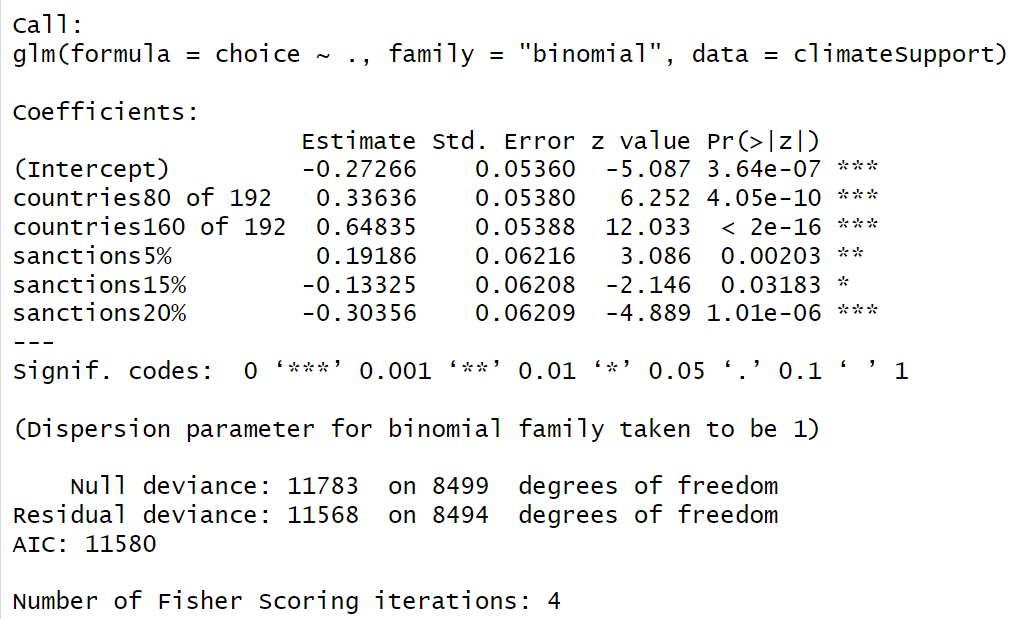
\includegraphics[width=0.7\textwidth]{Q1.png}\\
		Intercept indicates that when all independent variables are 0, the estimated logarithmic probability of the dependent variable is -0.27266.\\
		The estimated value of countries80 of 192 is 0.33636, indicating that when a country is one of 80 out of 192 countries, the logarithmic probability of the dependent variable increases by 0.33636.\\
		The estimated value of countries 160 of 192 is 0.64835, indicating that when a country is one of 160 out of 192 countries, the logarithmic probability of the dependent variable increases by 0.64835.\\
		The estimated value of sanctions5\% is 0.19186, indicating that when the severity of sanctions is 5\%, the logarithmic probability of the dependent variable increases by 0.19186.\\
		The estimated value of sanctions15\% is -0.13325, indicating that when the severity of sanctions is 15\%, the logarithmic probability of the dependent variable decreases by 0.13325.\\
		The estimated value of sanctions20\% is -0.30356, indicating that when the degree of sanctions is 20\%, the logarithmic probability of the dependent variable decreases by 0.30356.\\
		From the results, it can be seen that the P-values of all coefficients are less than the commonly used significance level of 0.05. This means that all coefficients are significant, and we have sufficient evidence to reject the assumption that the coefficients are zero, meaning that their impact on the dependent variable is significant.\\
		\lstinputlisting[language=R, firstline=60,lastline=71]{PS2.R} 
		\textbf{Result}:\\
		Global null hypothesis: 11783.41 \\
		Model p-value: 3.635432e-07 4.051815e-10 2.397037e-33 0.002025651 0.0318345 1.014753e-06 \\
		Global null hypothesis p-value: 0 \\
		In this model, the global null hypothesis is that all coefficients of the explanatory variables are equal to zero, indicating no influence of any explanatory variable on the outcome.\\
		According to the provided results, the p-value for the global null hypothesis is 0, indicating that we can reject the global null hypothesis.\\
		\lstinputlisting[language=R, firstline=97,lastline=111]{PS2.R} 
		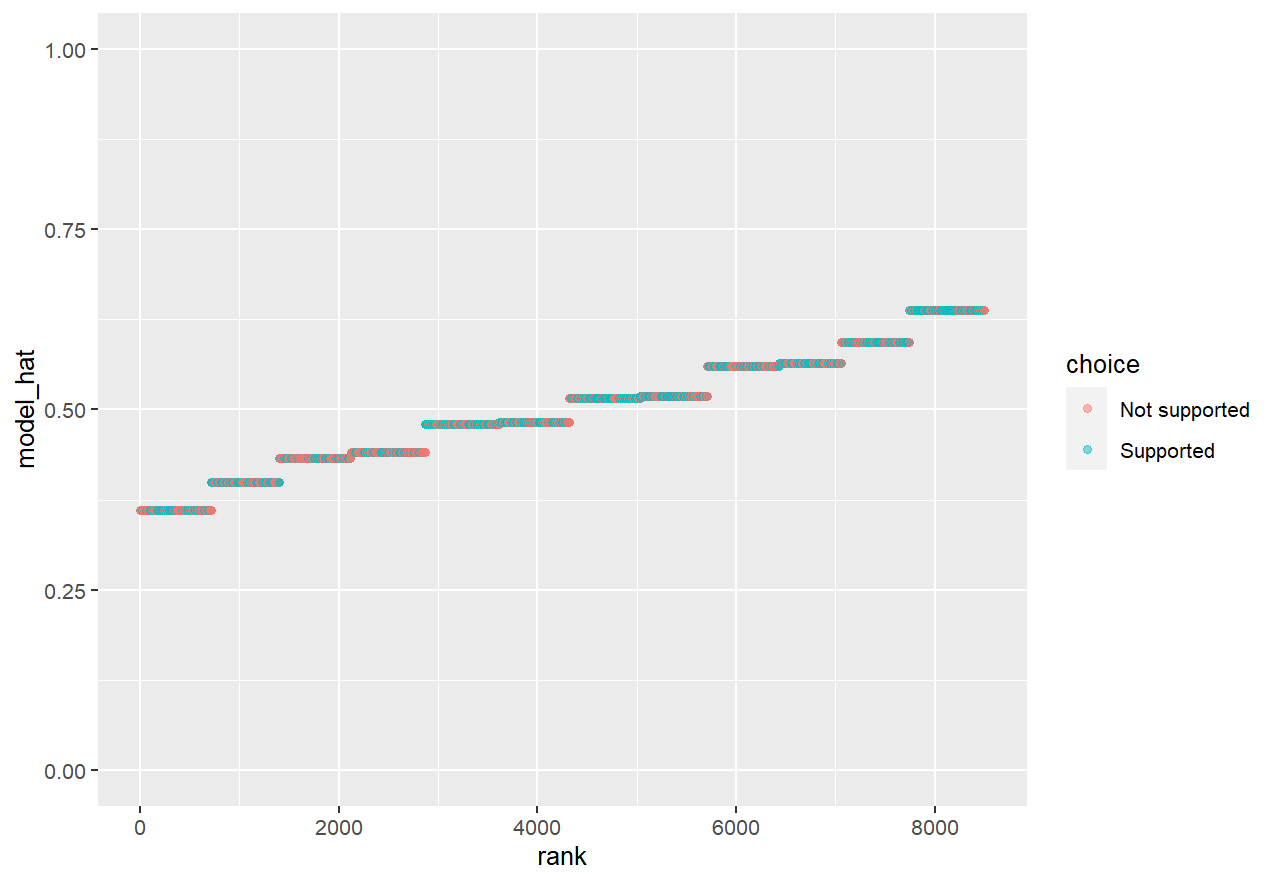
\includegraphics[width=0.8\textwidth]{Q1_1.png}\\
		
	\end{enumerate}
	
	\item
	If any of the explanatory variables are significant in this model, then:
	\begin{enumerate}
		\item
		For the policy in which nearly all countries participate [160 of 192], how does increasing sanctions from 5\% to 15\% change the odds that an individual will support the policy? (Interpretation of a coefficient)\\
		\lstinputlisting[language=R, firstline=72,lastline=85]{PS2.R} 
		\textbf{Result}:\\
		As sanctions increase from 5\% to 15\%, the probability of individuals supporting policies changes as follows: 0.7224531 \\
		\item
		What is the estimated probability that an individual will support a policy if there are 80 of 192 countries participating with no sanctions? \\
		\lstinputlisting[language=R, firstline=86,lastline=89]{PS2.R} 
		\textbf{Result}:\\
		Estimated probability of 80 countries without sanctions: 0.5159191 \\
		\item
		Would the answers to 2a and 2b potentially change if we included the interaction term in this model? Why? \\
		
		\begin{itemize}
			\item Perform a test to see if including an interaction is appropriate.
			\lstinputlisting[language=R, firstline=90,lastline=96]{PS2.R} 
			\textbf{Result}:\\
			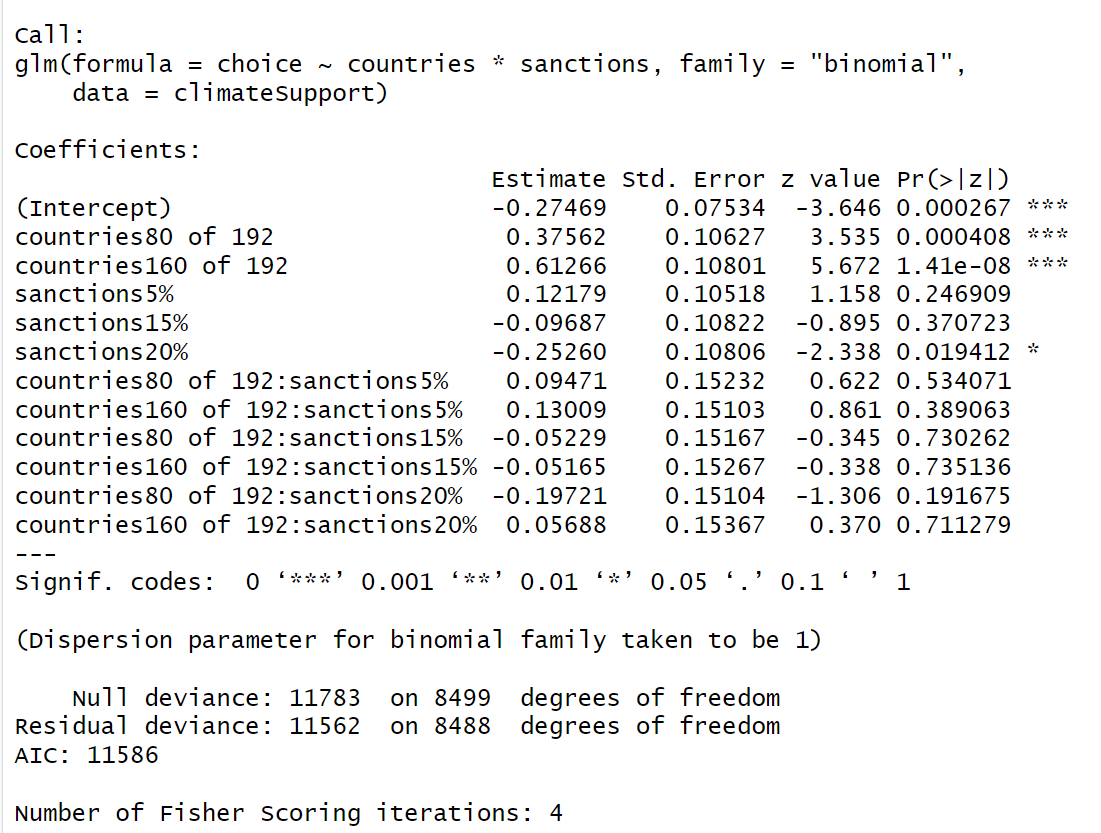
\includegraphics[width=0.8\textwidth]{Q2c1.png}\\
			\\
			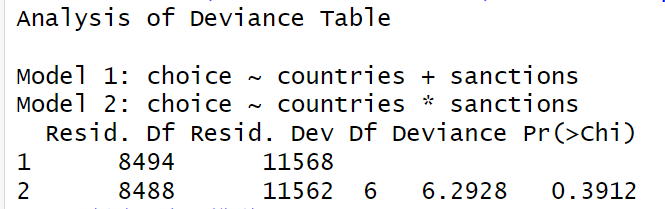
\includegraphics[width=0.6\textwidth]{Q2c2.png}\\
			The chi-square statistic between the two models is 6.29, with 6 degrees of freedom and a p-value of 0.39. This p-value suggests that we cannot reject the possibility that the difference between the two models is due to randomness, and therefore it can be argued that the inclusion of an interaction term in the model is unnecessary. So in this case it is not appropriate to add an interaction term and therefore there will be no change in the answers for 2a and 2b.\\
		\end{itemize}
	\end{enumerate}
	\end{enumerate}


\end{document}
